
\documentclass[conference, a4paper]{IEEEtran_ID}
\IEEEoverridecommandlockouts
\usepackage{cite}
\usepackage{fancyhdr}
\usepackage{lastpage}
\usepackage{amsmath,amssymb,amsfonts}
\usepackage{algorithmic}
\usepackage{graphicx}
\usepackage{textcomp}
\usepackage{xcolor}
\usepackage{listings}
\lstset { %
    language=C++,
    backgroundcolor=\color{black!5}, % set backgroundcolor
    basicstyle=\footnotesize,% basic font setting
}

\def\BibTeX{{\rm B\kern-.05em{\sc i\kern-.025em b}\kern-.08em
    T\kern-.1667em\lower.7ex\hbox{E}\kern-.125emX}}

\pagestyle{fancy}
\fancyhf{}
\lhead{}
\rhead{\footnotesize{COMPSCI 532 -- Fall 2020}}
\lfoot{}
\rfoot{\thepage { /} \pageref{LastPage}}
\renewcommand{\headrulewidth}{0pt}
\renewcommand{\footrulewidth}{0pt}


\begin{document}

\title{Map Reduce \\ 
\LARGE{COMPSCI 532 Project 1}
}

\author{
\IEEEauthorblockN{Vishal Keshav, Kenneth Myers, Jessie Huo} %\vspace{0.5em}
\IEEEauthorblockN{University of Massachusetts Amherst}
%\IEEEauthorblockN{}
}

\maketitle
\thispagestyle{fancy}


\section{Abstract}
In this report we discuss an implementation of MapReduce\cite{mapreduce} system and the technical challenges we faced along the way. MapReduce is a distributed computing paradigm where user-defined map and reduce functions are invoked in a large scale distributed system. Each data point is transformed (mapped) and the results are then collated (reduced). The framework takes care of how to distribute the tasks among servers and also how to tolerate the faults when a server stops responding. For detailed discussion on MapReduce, please refer to the original paper. Herein, however, we will discuss the over-all design, some implementation details and the APIs we have exposed to make distributed MapReduce possible. Furthermore, we also describe some of the design principals that enabled us to implement MapReduce system in a low level language, which in our case is C++.
 

\section{Design}
At the top level, clients only interact with a master module, communicate what needs to be done (such as where is the data and what are the map and reduce functions), there-after, the master orchestrate the map task and reduce task among the worker modules. Internally, the master controls how many worker (in a separate process) to invoke and how many threads per worker is allowed to run. Master also implements mechanism to detect and recover the faulty worker.

\begin{figure}[htbp]
		\centerline{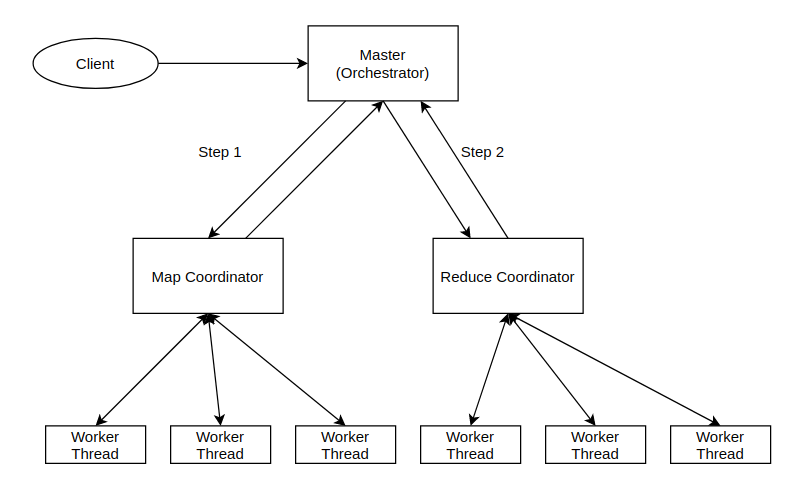
\includegraphics[width=0.49\textwidth]{high_level_design.png}}
		\caption{A high level design is shown}
\end{figure}

We deal with a system where all workers have access to the database (either through a shared mechanism or through the network file system). We also assume that if the master fails, then the client will know and invoke the master again. However, if one worker fails, the master will recover that worker. We only deal with the failure of at most one map and one reduce worker during map-reduce process.

The master module is a class called MapReduceMaster that the client program must instantiate. The client program is also required to implement the map and reduce user-defined functions (UDF) in a class that is inherited from the MapReduceInterface. Once the client program registers the interface, then the map reduce program becomes aware of the map and reduce functionality.

The interaction diagram is shown below:
\begin{figure}[htbp]
		\centerline{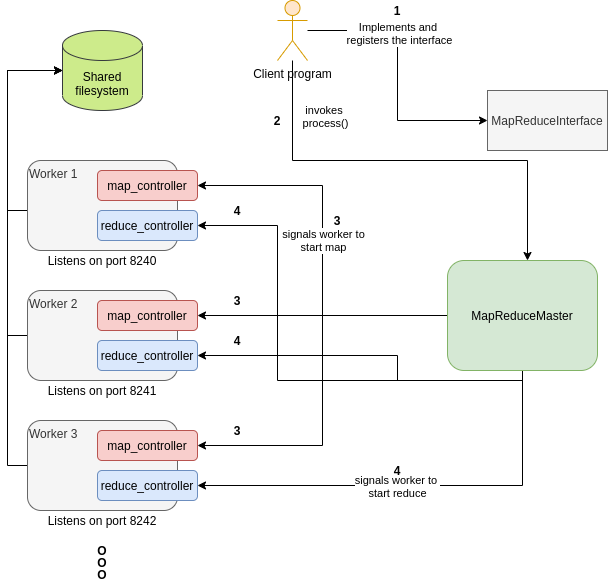
\includegraphics[width=0.49\textwidth]{interaction_diagram.png}}
		\caption{Interaction diagram for MapReduce}
\end{figure}
\section{Interface}
In this section, we detail the MapReduce APIs through a sample program WordCounter. The first step is to include the "only header" MapReduce library header into the program.
\begin{lstlisting}
#include "MapReduceMaster.h"
\end{lstlisting}

The client program then publicly inherits the \textit{MapReduceInterface} class and must implements two functions namely \textit{map\_fn} and \textit{reduce\_fn}. The \textit{map\_fn} defines how a function is applied to each iterable in the data, such as a line in a file. It must call an inherited method \textit{emitIntermediate(intermediate\_key, value)} which will push the intermediate key and it’s corresponding value to an array (used by MapReduce program internally and described later on). Similarly the \textit{reduce\_fn} must define how to reduce a key and all of the values associated with that key. It must call \textit{emit(key, value)} which will push the reduced key-value pair to another array. 

\begin{lstlisting}
class WordCounterMapReduce:public MapReduceInterface
{
public:
    void map_fn(string key, string value)
    {
        stringstream iss(value);
        string word;
        while (iss >> word) {
            emitIntermediate(word, "1");
        }
    }

    void reduce_fn(string key,vector<string> values)
    {
        int count = 0;
        for (int i =0; i<values.size(); i++) {
            count += stoi(values[i]);
        }
        emit(key, vector<string>{to_string(count)});
    }
};
\end{lstlisting}
Please note that the client program does not need to define the \textit{emitIntermediate} and \textit{emit} functions, as they are implemented by the base class \textit{MapReduceInterface} but they must be called by the user..

Once this is done, the client then registers the \textit{MapReduceInterface} to the MapReduce program. This registration follows a design principal called Factory because C++ does not support reflection, which is quite common in other languages like Java. The registration enables the \textit{MapReduceMaster} to recognize the map and reduce function, which it then internally uses across the map and reduce worker servers. The code to register the interface is shown below:
\begin{lstlisting}
MapReduceInterfaceFactoryRegistration \
    <WordCounterMapReduce> \
        _WordCounterMapReduce("MapReduce");
\end{lstlisting}

The third and final step is to create an object of type \textit{MapReduceMaster} and invoke the \textit{process()} function on it.
\begin{lstlisting}
int main() {
    int nr_workers = 2;
    string inputFileName = "input.txt";
    string dataDirectory = "DataDirectory";

    MapReduceMaster masterInstance(
                inputFileName,
                dataDirectory,
                nr_workers);
    int result = masterInstance.process();
    return 0;
}
\end{lstlisting}
Please note the APIs. The constructor of \textit{MapReduceMaster} has three arguments, namely which text file is to be processed, in which directory the input file lies and how many workers per map and reduce are requested. The data directory is where the map reduce program produces the output.txt as well as temp.txt files. Note that, based on the number of workers selected, the output and temporary files may differ as they would then be output\_[i].txt where i is the reduce worker index and temp\_[i]\_[j].txt where i is map worker index and j is reduce worker index.

\section{Implementation details}
Having defined the APIs, we now discuss some internal details of the MapReduce program itself.

\subsection{Remote procedure calls}
To enable the remote procedure calls(RPC), we rely on a C++ based RPC library \cite{rpc}. This library allows us to get rid of cumbersome low level socket programming. However, the way this library handles the remote calls is quite primitive and low level. Hence, we build on the library to implement our own remote protocols. We register five main functions to each server we spawn in a separate process. They are \textit{map\_controller\_module}, \textit{reduce\_controller\_module}, \textit{exit}, \textit{is\_map\_done} and \textit{is\_reduce\_done}. Each of these will be discussed in later sections.

\subsection{Fault tolerance and heart-beat mechanism}
The fault tolerance is implemented to withstand at-most one map worker and one reduce worker failure. To detect if there is a server failure, the master continuously polls a global variable from each server. These variables are polled by calling the function \textit{is\_map\_done} during map phase and \textit{is\_reduce\_done} during reduce phase. The calls are non-blocking because each server handles this request in a different thread while continuing the map or reduce task in a different thread. Moreover, master sleeps for 1 seconds before polling each of the servers again.

In each loop, the master also checks if the server listening on different ports (the ports used in the MapReduce program) are still alive. This is done just by checking if master can still bind to a particular port. If it still can before the task is completed, then the server is faulty and the fault recovery mechanism is followed.

To recover from the server fault, the master again spawns a process (with two threads) on the same port where the server is able to listen again.

\section{Controller implementation}
As mentioned previously, the master binds a number of functions to each worker and these tasks include \textit{map\_controller\_module} and a \textit{reduce\_controller\_module}. 
\subsection{Map controller module}

The execution of the map and reduce tasks are aided by two additional functions, \textit{map\_controller\_module} and \textit{reduce\_controller\_module}. The \textit{map\_controller\_module} scans each line of the file and reads the line if a particular line hashes to the mapper that is scanning the file. Then the registered map function is applied to the line. Note that, even if lines are scanned, it is not read unless required by the corresponding mapper. In C++, there is no way to read the bytes of the file unless someone breaks the input file into parts (which again will scan through the file to at-least know how many lines there are in the file).

Then it creates a temp file to store each of the intermediate key-value pairs pushed to an array by the interface. Each of these files has the form "temp\_[mapper\_id]\_[reducer\_id].txt" where mapper\_id corresponds to the current worker and reducer\_id corresponds to the reduce worker ID where this file will end up for reduce task. Finally the module loops over all of the emitted intermediate key-value pairs, hashes each to a reduce worker based on the intermediate key and writes that pair to the associated temp file. No extra work per map worker is done in the whole process.

\subsection{Reduce controller module}

The \textit{reduce\_controller\_module} provides analogous support. It begins by searching for temp files with its associated id, for example worker 2 will look for all temp files that look like “temp\_[mapper\_id]\_2.txt”. It then loops over the contents of each file and builds a mapping of each key and an array of their associated values. It then loops over each key-value in the mapping and applies the user-defined \textit{reduce\_fn} from the interface on each of these pairs which emits the result to an array via the \textit{emit} method. Finally it writes each of the reduced key-value pairs that were pushed to the array to an output file associated with the reducer, "output\_[reducer\_id].txt".

\section{Evaluation}
To simplify the correctness of the systems, we have done the following:
\begin{itemize}
    \item Provided a comprehensive README.md that details and demonstrates the behaviour of the programs with Map Reduce library. Please see the screen captures embedded in the README.md
    \item Implemented three programs namely WordCounter, InvertedIndex and ReverseWeblinkGraph and created a corresponding small data sets on which these programs operate. The correctness the of the generated output can be visually verified.
    \item Implemented the spark programs for WordCounter, InvertedIndex and ReverseWeblinkGraph, the output of which will be generated along with the output of the the program we implemented with Map reduce library.
    \item Created a script that build the three programs and also runs the spark programs, generates all outputs in the build directory, which can be visually verified, as our data sets are small.
    \item The programs uses more than one mapper and reducer to demonstrates the scalability of the Map reduce library. However, once the programs are compiled, those programs can still be used to process a different and probably larger dataset on many worker thread by only modifying the configuration file. Look for the config\_WordCounter.txt and similary for others in the build directory.
\end{itemize}

Here we provided a single command that can be used to build and run everything in one step.
\begin{lstlisting}
sh script.sh
\end{lstlisting}
This command automatically copies the relevant data from relevant directories and put them in the build directory, where the rest of the program are compiled and outputted.
For more details, refer to the README.md.


\section{Conclusion}
We have implemented the MapReduce program in C++ which support distributed processing, fault tolerance up to one map and reduce worker. Our implementation is constrained by processing a single shared file, however this constraint too can be removed by little workaround.


% see file Documentation.bib
\bibliographystyle{IEEEtran}
\bibliography{Proposal}

\end{document}